% =============================================================================
% CHAPTER 5: Design and Implementation
% =============================================================================
% SPDX-FileCopyrightText: 2026 Drewan Rutherford <RutherfordD@cardiff.ac.uk>
% SPDX-License-Identifier: LPPL-1.3c
% =============================================================================

This chapter details some of the systems developed for the prototype, namely:

\begin{enumerate}
    \item CatBot, the player,
    \item The CatCode back-end, the fictional programming language developed for this game,
    \item Graphical CatCode, the GUI systems for the programming GUI.
\end{enumerate}

Where possible source-code files will be referenced. \textquote{\texttt{.tscn}} are scene files, it is recommended that you view these in the Godot editor, and \textquote{\texttt{.gd}} are GDscript files, which can be viewed either in the editor or an text-editor of your choice.

The project uses Godot version 4.6.2 \citep{Godot4.6}, at time of submission, because it was the latest stable version available.

This report assumes that you are familiar with the many Godot, GDscript and their many quirks. Whilst completely independent from python, GDscript is somewhat similar to python being duck-typed (unless variable types are specified), indent-based, with variables being public \citep{GDscriptReference}. Links to the GDscript reference, Godot 4.6  and its documentation are in \autoref{tab:design/godotLinks}.

\begin{figure}[]
    \centering
    \begin{tabular}{r|p{10cm}}
        Godot Website & \url{https://godotengine.org/} \\
        Download & \url{https://godotengine.org/download/archive/} \\
        Source Code & \url{https://github.com/godotengine/godot/tree/4.6} \\
        4.6 Documentation & \url{https://docs.godotengine.org/en/4.6/} \\
        4.6 GDscript reference & \url{https://docs.godotengine.org/en/4.6/tutorials/scripting/gdscript/gdscript_basics.html} \\
    \end{tabular}
    \caption{Links to the Godot engine and its resources}
    \label{tab:design/godotLinks}
\end{figure}

Stylistically, this game uses pixel art in combination with full resolution UI. The pixel art is partially as a throwback to retro games such as the NES game Super Mario Bros \citep{SMB-NES} -- though strict limits such colour palette sizes were not maintained, and partially for more practical reasons such as time constraints and to keep file sizes low to aid with storage and memory use. 

\break

\section{CatBot}\label{sec:design/catBot}

The character controlled by the player is CatBot: a robot that looks like the cat, that has a failing control system that constants needs fixing. A cat was chosen as a combination for a few reasons. First, the developer is good, and enjoys, drawing cats. Second, cats are popular companions with an estimated 10.2 million pet cats in the UK \citep{CatOwnership}. And, finally, but more importantly, the developer had an existing sprite-sheet, shown in  that could be re-used, alongside an existing system that could be used as a base.

\begin{figure}
    \centering
    \begin{subfigure}[t]{0.45\linewidth}
        \centering
        
\includegraphics[width=1\linewidth]{C5/CatBot/Jumping.png}
        \caption{CatBot jumping}
    \end{subfigure}
    \begin{subfigure}[t]{0.45\linewidth}
        \centering
        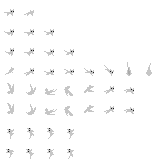
\includegraphics[width=0.75\linewidth]{C5/CatBot/SpriteSheet.png}
        \caption{Sprite-sheet}
    \end{subfigure}
    \caption[CatBot and CatBot's sprite-sheet]{CatBot and CatBot's sprite-sheet, available in \texttt{res://assets/player/Kitis.png}. Only rows 1 -- 4 were used for CatBot.}
    \label{fig:design/catBotSpriteSheet}
\end{figure}

CatBot (found in \texttt{res://src/entities/player/player\_cat.tcsn}), which extends the custom-made \texttt{generic\_entity} class (...\texttt{/classes/generic\_entity.gd}). \texttt{generic\_entity} provides basic functions such managing HP, stability, and typing\footnote{Godot default type methods only provide the node type. Providing this method as a base to all entities makes implementing future systems easier}; and, in turn, extends the built-in \href{https://docs.godotengine.org/en/stable/classes/class\_characterbody2d.html}{Character Body 2D} node. This provides numerous functions, such as \texttt{move\_and\_slide()}, and attributes such as \texttt{velocity} that aid with entities with custom dynamic physics.

The structure of the CatBot scene is shown in \autoref{fig:design/catBot-NodeStructure}.

\begin{figure}
    \centering
    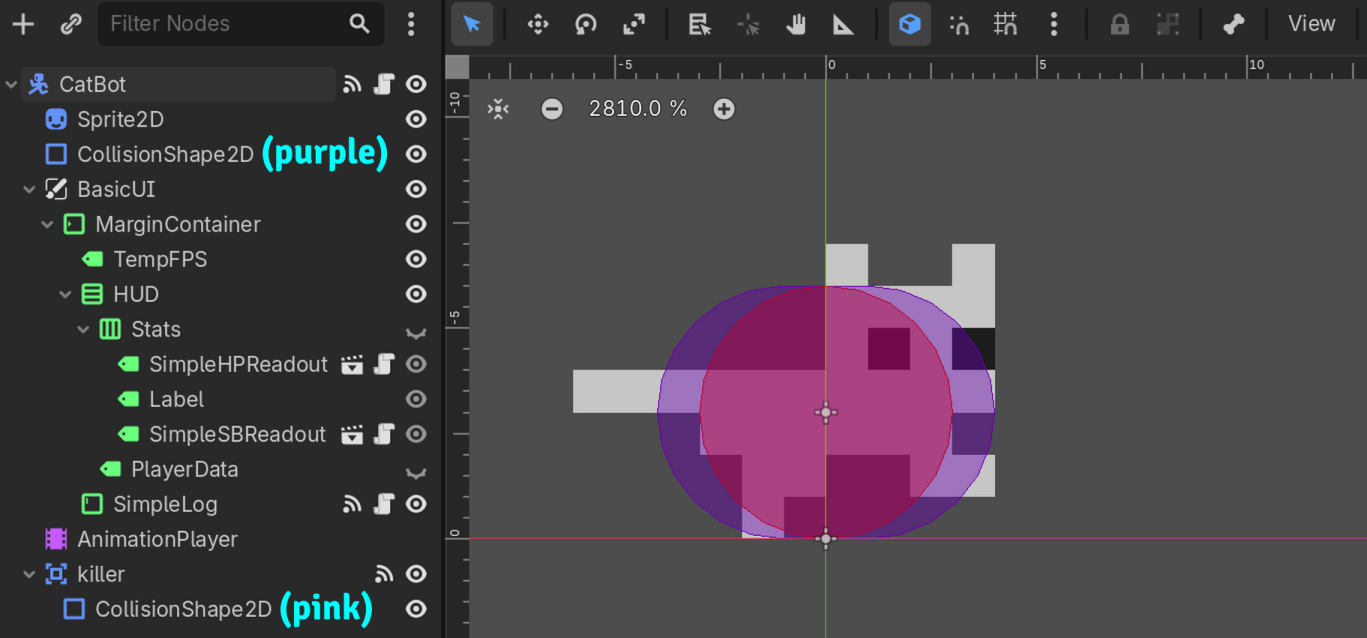
\includegraphics[width=0.75\linewidth]{C5//CatBot/nodeStructure.png}
    \caption[CatBot node structure]{CatBot node structure}
    \label{fig:design/catBot-NodeStructure}
\end{figure}



\section{CatCode Back-end}\label{sec:design/catCodeBackend}

nyah meow purrr

\section{Graphical CatCode}\label{sec:design/catCodeFrontend}

Nyah meow purrr

